%Preamble
\documentclass[12pt]{article}
\usepackage{fancyhdr}
\usepackage{extramarks}
\usepackage{amsmath}
\usepackage{amssymb}
\usepackage{amsthm}
\usepackage{amsrefs}
\usepackage{amsfonts}
\usepackage{mathrsfs}
\usepackage{mathtools}
\usepackage[mathcal]{eucal} %% changes meaning of \mathcal
\usepackage{enumerate}
\usepackage[shortlabels]{enumitem}
\usepackage{verbatim} %% includes comment environment
\usepackage{hyperref}
\usepackage[capitalize]{cleveref}
\crefformat{equation}{~(#2#1#3)}
\usepackage{caption, subcaption}
\usepackage{graphicx}
\usepackage{fullpage} %%smaller margins
\usepackage[all,arc]{xy}
\usepackage{mathrsfs}

\hypersetup{
    linktoc=all,     % set to all if you want both sections and subsections linked
}

\topmargin=-0.45in
\evensidemargin=0in
\oddsidemargin=0in
\textwidth=6.5in
\textheight=9.0in
\headsep=0.25in
\setlength{\headheight}{16pt}

\linespread{1.0}

\pagestyle{fancy}
\lhead{\Name}
\chead{\hwClass: \hwTitle}
\rhead{\hwDueDate}
\lfoot{\lastxmark}
\cfoot{\thepage}

\renewcommand\headrulewidth{0.4pt}
\renewcommand\footrulewidth{0.4pt}

\setlength\parindent{0pt}

%% Title Info
\newcommand{\hwTitle}{HW \# 3}
\newcommand{\hwDueDate}{Feb 1, 2020}
\newcommand{\hwClass}{AMATH 585}
\newcommand{\hwClassTime}{}
\newcommand{\hwClassInstructor}{}
\newcommand{\Name}{\textbf{Marlin Figgins}}


%% MATH MACROS
\newcommand{\bbF}{\mathbb{F}}
\newcommand{\bbN}{\mathbb{N}}
\newcommand{\bbQ}{\mathbb{Q}}
\newcommand{\bbR}{\mathbb{R}}
\newcommand{\bbZ}{\mathbb{Z}}
\newcommand{\bbC}{\mathbb{C}}
\newcommand{\abs}[1]{ \left| #1 \right| }
\newcommand{\diff}[2]{\frac{d #1}{d #2}}
\newcommand{\infsum}[1]{\sum_{#1}^{\infty}}
\newcommand{\norm}[1]{ \left|\left| #1 \right|\right| }
\newcommand{\eval}[1]{ \left. #1 \right| }
\newcommand{\Expect}[1]{\mathbb{E}\left[#1 \right]}
\newcommand{\Var}[1]{\mathbb{V}\left[#1 \right]}
\renewcommand{\vec}[1]{\mathbf{#1}}

\renewcommand{\phi}{\varphi}
\renewcommand{\emptyset}{\O}

%--------Theorem Environments--------
%theoremstyle{plain} --- defaultx
\newtheorem{thm}{Theorem}[section]
\newtheorem{cor}[thm]{Corollary}
\newtheorem{prop}[thm]{Proposition}
\newtheorem{lem}[thm]{Lemma}
\newtheorem{conj}[thm]{Conjecture}
\newtheorem{quest}[thm]{Question}

\theoremstyle{definition}
\newtheorem{defn}[thm]{Definition}
\newtheorem{defns}[thm]{Definitions}
\newtheorem{con}[thm]{Construction}
\newtheorem{exmp}[thm]{Example}
\newtheorem{exmps}[thm]{Examples}
\newtheorem{notn}[thm]{Notation}
\newtheorem{notns}[thm]{Notations}
\newtheorem{addm}[thm]{Addendum}

% Environments for answers and solutions
\newtheorem{exer}{Exercise}
\newtheorem{sol}{Solution}

\theoremstyle{remark}
\newtheorem{rem}[thm]{Remark}
\newtheorem{rems}[thm]{Remarks}
\newtheorem{warn}[thm]{Warning}
\newtheorem{sch}[thm]{Scholium}

\makeatletter
\let\c@equation\c@thm
\makeatother

\begin{document}

\begin{exer}
    \begin{enumerate}[(a)]
        \item Write a program to solve the boundary value problem for the nonlinear pendulum as discussed in the text. See if you can find yet another solution for the boundary conditions illustrated in Figures 2.4 and 2.5.
        \item Find a numerical solution to this BVP with the same general behavior as seen in Figure 2.5 for the case of a longer time interval, say, $T = 20$, again with $\alpha = \beta = 0.7$. Try larger values of T. What does $\max_{i} \theta_{i}$ approach as $T$ is increased? Note that for large $T$ this solution exhibits “boundary layers”.
    \end{enumerate}
\end{exer}


\begin{sol}

    (a) We solve the BVP for the non-linear pendulum. Trying a random sampling of 20 initial guess, we arrive at the three solutions pictured below.


    (b) Tweaking the grid size and $T$, we arrive at several solutions which appear to increase in height. From this, I would guess that $\max_{i} \theta_{i}$ approaches infinity as $T$ increases. Plots are embedded below.
\end{sol}
\begin{figure}[h]
    \centering
    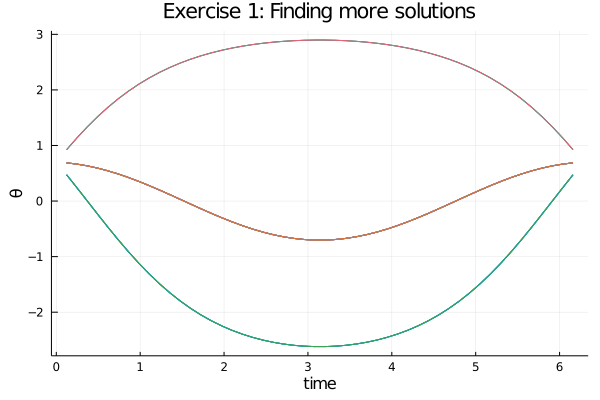
\includegraphics[width=0.8\linewidth]{figs/hw-3-exer1-more-sol.png}
    \caption{Finidng more solutions with random sampling of initial guesses.}%
    \label{fig:figs/hw-3-exer1-more-sol}
\end{figure}


\newpage

\begin{figure}[h]
    \centering
    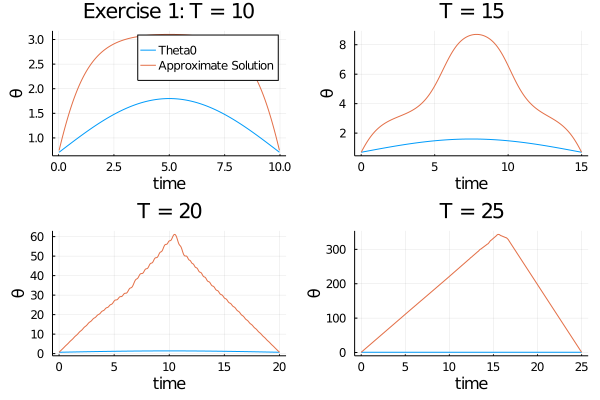
\includegraphics[width=0.8\linewidth]{figs/hw-3-max-theta.png}
    \caption{Solutions of the pendulum problem as $T$ increases.}
    \label{fig:figs/hw-3-max-theta}
\end{figure}

\newpage

\begin{exer}[ Gerschgorin’s theorem and stability ]
    Consider the boundary value problem
    \begin{align*}
        - u_{xx} + (1 + x^{2}) u = f, 0\leq x \leq 1,\\
        u(0) = 0, u(1) = 0.
    \end{align*}
    On a uniform grid with spacing $h = \frac{1}{m+1}$, the following set of difference equations has local truncation error $O(h^{2})$:
    \begin{equation*}
        \frac{2 u_{i} - u_{i+1} - u_{i-1}}{h^{2}} + (1 + x_{i}^{2})u_{i} = f(x_{i}), i = 1, \ldots, m.
    \end{equation*}
    (a) Use Gerschgorin's theorem to determine upper and lower bounds on the eigenvalues of the coefficient matrix for this set of difference equations.
    (b) Show that the $L_{2}$-norm of the global error is of the same order as the local truncation error.
\end{exer}


\begin{sol}
    Using Gerschgorin's theorem, we bound the eigenvalues of the coefficient matrix $A$ as follows. Each row has entries of the form
    \begin{align*}
        A_{i-1,i} &= - \frac{1}{h^{2}}\\
        A_{i,i} &= \frac{2}{h^{2}} + x_{i}^{2} + 1\\
        A_{i,i+1} &= - \frac{1}{h^{2}},
    \end{align*}
    so that the eigenvalues live in disks of the form
    \begin{equation*}
      D_{i} = \left\{ z \in \bbC \colon \abs{z - \left(\frac{2}{h^{2}} + x_{i}^{2} + 1 \right)} \leq \frac{2}{h^{2}} \right\}.
    \end{equation*}
    We can simplify this inequality for any $i$ as follows
    \begin{equation*}
    1 + x_{i}^{2} \leq \lambda \leq \frac{4}{h^{2}} + 1 + x_{i}^{2}.
    \end{equation*}
    With the knowledge that $x_{i} \in [0,1]$, we have that any eigenvalue has
    \begin{equation*}
    1 \leq \lambda \leq 2 + \frac{4}{h^{2}}.
    \end{equation*}
    Therefore, we have that 
    \begin{equation*}
        \norm{A^{-1}}_{2} = \left(\min_{i} \abs{ \lambda_{i} } \right)^{-1} \approx 1
    \end{equation*}
    where $\lambda_{i}$ are the eigenvalues of $A$. As we can see this norm does not depend on $h$ due to the minimum we've derived above. Therefore, we have that the $L_{2}$ norm of the global error is bounded by
    \begin{equation*}
        \norm{ E }_{2} \leq \norm{A^{-1}}_{2} \norm{ \tau }_{2} \approx \norm{\tau }_{2}
    \end{equation*}
  i.e. the $L_{2}$ norm of the global error is on the same order as the local truncation error.
\end{sol}

\newpage

\begin{exer}[Richardson extrapolation]
    Use your code from problem 6 of assignment 1 to do the follow exercise. Run the code with $h = .1$ (10 subintervals) and with $h = 0.05$ (20 subintervals) and apply Richardson extrapolation to obtain more accurate solution values on the coarser grid. Record the $L_{2}$-norm or the $\infty$-norm of the error in the approximation obtained with each $h$ value and in that obtained with extrapolation.

    Suppose that you assume the coarse grid approximation is piecewise linear, so that the approximation at the midpoint of each subinterval is the average of the values at the two endpoints. Can one use Richardson extrapolation with the fine grid approximation and these interpolated values on the coarse grid to obtain a more accurate approximation at these points? Explain why or why not?
\end{exer}


\begin{sol}
Using the $L_{2}$ norm, we see that the $L_{2}$ error for $h = .1$ is $ 2.0 \times 10^{-3}$, $h = .2$ is $5 \times 10^{-5}$, and the error is $9.5 \times 10^{-6}$ for the Richardson extrapolation.


I'm a bit unclear on what this is asking, so I'll rephrase the question a bit and answer it as I understand it. If the question is asking whether it is possible to compute linearly interpolated  values between elements on a coarse grid and combine these interpolated values along with the value of the approximation on a finer grid to get a better approximation at an element on the fine grid, I would say yes. 


Suppose that we have a function $f$ which is being linearly interpolated between points $x_{0}$ and $x_{2} = x_{0} + 2h$. Then we have that the error on this interval can be written as
\begin{equation*}
    E(x) = f(x) - \left(  f(x_{0}) + \frac{f(x_{2}) - f(x_{0})}{x_{2} - x_{0}} (x - x_{0})\right).
\end{equation*}
Expanding $f(x)$ around $x_{1} = x_{0} + h$, we see that this is on the order
\begin{align*}
    E(x_{1}) &\approx f'(x_{1}) h - \frac{f(x_{2}) - f(x_{0})}{x_{2} - x_{0}}h + O(h^{2})\\
             &= \left( f'(x_{1}) - \frac{f(x_{1} + h) - f(x_{1} - h)}{2h} \right) h + O(h^{2})
\end{align*}
Noting the centered difference approximation of the first derivative is on the order of $O(h^{2})$, we see that the error of the approximation is on the order of $O(h^{2})$. From this argument, I believe we could combine the above estimates of $x_{1}$ using $h$ and $h / 2$ in a Richardson approximation to approximate $x_{1}$ at a higher order. Though this is still  distinct from what has been asked.


As we've seen the linear interpolation at the midpoint on the coarse grid should be on the order of $O(h^{2})$ which is the same as the order of the value computed on finer grids method. Specifically using Richardson extrapolation, this doesn't fit because it relies on using the fact that we are using the same general method to generate our approximations I do think it may be possible to make another approximation though since the methods have the same order accuracy by taking something like
\begin{equation*}
    \frac{\lambda_{1} A(h / 2) - \lambda_{2} B(h)}{\lambda_{3}},
\end{equation*}
where $A( h / 2 )$ denotes the approximation on the finer grid and $B(h)$ is the linear interpolation and the $\lambda$ are picked to cancel out the coefficient of order $O(h^{2})$.
\end{sol}

\newpage

\begin{exer}
Write down the Jacobian matrix associated with Example 2.2 and the nonlinear difference equations (2.106) on p. 49. Write a code to solve these difference equations when $a=0$,$b=1$, $\alpha=-1$,$\beta=1.5$,and $\epsilon=0.01$. Use an initial guess of the sort suggested in the text. Try $h=1 / 20$, $h=1 / 40$, $h=1 / 80$,and $h=1 / 160$, and turn in a plot of your results.
\end{exer}

\begin{sol}
    Computing the Jacobian associated with example 2.2, we get 
    \begin{align*}
        \frac{\partial G_{i}(U)}{\partial U_{i-1}} &= \frac{\epsilon}{h^{2}} - \frac{U_{i}}{2h} \\
        \frac{\partial G_{i}(U)}{\partial U_{i}}  &= -\frac{2\epsilon}{h^{2}} + \left( \frac{U_{i+1} - U_{i-1}}{2h} - 1\right)\\
        \frac{\partial G_{i}(U)}{\partial U_{i+1}} &= \frac{\epsilon}{h^{2}} + \frac{U_{i}}{2h}
    \end{align*}

    Implementing this in julia for various step sizes, we get the below figure. Notice the oscillatory behavior near the interior layer. Steps sizes less than $ 0.05$ appear to remedy this behavior which is consistent with the estimate described by (2.108).
\end{sol}

\begin{figure}[ht]
    \centering
    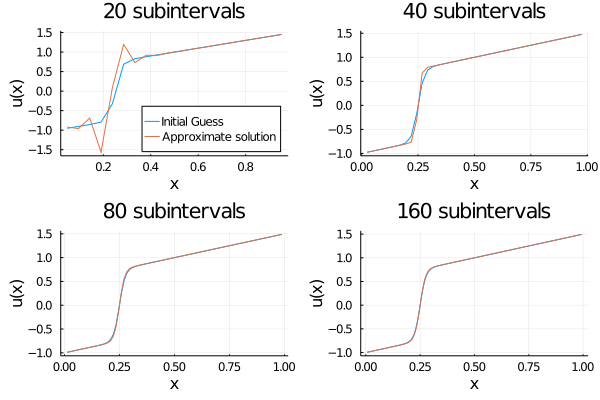
\includegraphics[width=0.8\linewidth]{figs/hw-3-exer-4.png}
    \caption{Solution of difference equations from exercise 4 using Newton's method.}
    \label{fig:figs/hw-3-exer-4}
\end{figure}
\newpage
\end{document}
